% Provenance (never printed): see sources/outline_sources.md (Year 3:
% radial velocity, transits, imaging and microlensing; what has been
% found; atmospheres from transmission spectra).
% Brief: sources/book5/BRIEFS.md, ch. 28. Curves from figdata/bachelor-3/
% rv_transit.py (Keplerian radial-velocity curves, a limb-darkened transit
% light curve computed by numerical integration, point-lens microlensing)
% and exoplanet_archive.py (the NASA Exoplanet Archive's composite table of
% confirmed planets, fetched 2026-10-23, with the model mass--radius curves
% of Zeng et al.). Exercise and problem values in the Book 5 scratch
% calculator calc/ch28.py. Selene's Lamp and its planet are invented.
\chapter{系外行星}\label{ch:b3:exoplanets}

1994 年秋，两位天文学家测量 142 颗恒星的速度，
发现其中一颗恒星 51~Pegasi 时而朝向我们、时而远离我们运动，
周期约为四天。运动的半振幅为
\qty{59}{m.s^{-1}}，是光谱仪可探测量的四倍。
拉动该恒星运动的伴星，质量至少为木星的一半，
轨道半径为 \qty{0.05}{au}，离恒星的距离约为
水星离太阳距离的八分之一。行星形成理论原本没有给这类天体留下位置。
该发现于 1995 年 10 月公布，开辟了天文学的一个新领域：
三十年后，已确认的系外行星超过六千颗，
其中几颗已被直接观测到，部分行星的
大气已被分析。本章介绍如何找到那些太暗而无法直接看见的行星，
已发现的情况，以及它们的大气如何
被读取。
% ledger: nobel19:51peg, planet:Mercury.dist, data:b5-pscomp

\begin{recall}
多普勒效应、视向速度、分光双星、开普勒定律、二体问题及其
质心、普朗克定律，以及
等温大气的标高，已在物理学教材中学过。系外行星与恒星的
宜居带，已在中学教材中学过。通量与源的光度，
见于本科一年级分册中关于望远镜与测光的一章；平衡温度，
见于其中关于比较行星学的一章。行星形成与雪线，
见于本科二年级分册。\omterm{def:b3:planetary-atmospheres:jeans-escape}{金斯逃逸}与\omterm{def:b3:planetary-atmospheres:hydrodynamic}{流体动力学逃逸}，
以及宜居带的界限，
见于本科三年级分册中
关于行星大气的一章。
\end{recall}

\section{视向速度法}\label{sec:b3:exoplanets:rv}

行星并不绕恒星运行：二者都绕它们的公共质心运动。
恒星质量大得多，它沿一个很小的轨道运动，其光
随行星的周期在蓝移与红移之间往复变化。

\begin{definition}[视向速度法；最小质量]\label{def:b3:exoplanets:rv}
称\emph{视向速度法}\index{视向速度法}为：利用
恒星视向速度的周期性变化探测行星，
其视向速度由恒星光谱谱线的多普勒位移测得。当
轨道对天球平面的倾角 $i$ 未知时，它只能测得
行星质量与倾角正弦之积 $m_p\sin i$，
称该量为\emph{最小质量}\index{最小质量}，
即行星质量的下限。
\end{definition}

\begin{theorem}[视向速度半振幅]\label{thm:b3:exoplanets:semi-amplitude}
设质量为 $M_\star$ 的恒星与质量为 $m_p$ 的行星沿周期为
$P$、倾角为 $i$ 的圆轨道运动，则恒星的视向速度为
$v_r(t) = \gamma + K\cos\bigl(2\pi(t - t_0)/P\bigr)$，其中 $\gamma$ 为
质心的速度，半振幅为
\[
K = \left(\frac{2\pi G}{P}\right)^{1/3}
    \frac{m_p\sin i}{(M_\star + m_p)^{2/3}} .
\]
若轨道的偏心率为 $e$，曲线不再是正弦曲线，
此时 $v_r = \gamma + K\bigl[\cos(\nu + \omega) + e\cos\omega\bigr]$，其中 $\nu$
为真近点角，$\omega$ 为近星点幅角，且 $K$ 应
除以 $\sqrt{1 - e^2}$。
\end{theorem}

\begin{proof}
对圆轨道：两天体的距离 $a$ 满足
开普勒第三定律 $a^3 = G(M_\star + m_p)P^2/4\pi^2$。恒星位于
距质心的距离为 $a_\star = a\,m_p/(M_\star + m_p)$，
并以速率 $v_\star = 2\pi a_\star/P$ 沿其圆周运动。于是
\[
v_\star = \frac{2\pi}{P}\,\frac{m_p}{M_\star + m_p}
          \left(\frac{G(M_\star + m_p)P^2}{4\pi^2}\right)^{1/3}
        = \left(\frac{2\pi G}{P}\right)^{1/3}\frac{m_p}{(M_\star + m_p)^{2/3}} .
\]
\omterm{def:b3:remote-sensing-gis:insar}{视线方向}与轨道平面的夹角为 $\pi/2 - i$，
因此恒星速度中只有 $v_\star\sin i$ 一项沿\omterm{def:b3:remote-sensing-gis:insar}{视线方向}，
该分量随恒星一同变化：$v_r - \gamma = v_\star\sin i\,
\cos\bigl(2\pi(t - t_0)/P\bigr)$。偏心轨道的形式由
开普勒椭圆导出，在本阶段不加证明地承认。
\end{proof}

由于行星远比恒星轻，$K$ 即可确定 $m_p\sin i$，
在测得周期、并由光谱得知恒星质量之后，
对 51~Pegasi~b，$K = \qty{59}{m.s^{-1}}$，$P = \qty{4.23}{d}$，
恒星质量取一个太阳质量，则得 $m_p\sin i = 0.47$ 个木星质量。
木星使太阳以 \qty{12.5}{m.s^{-1}} 的速度运动，其轨道周期为
\num{4331} 天；远方的观测者会看到，太阳的速度在
十二年间摆动约 \qty{\pm 13}{m.s^{-1}}。地球使太阳运动的速度为
\qty{9}{cm.s^{-1}}。发现 51~Pegasi~b 的光谱仪可探测
\qty{13}{m.s^{-1}}；后继仪器可达约 \qty{1}{m.s^{-1}}（
相当于步行速度 \qty{3.5}{km/h}），最新的仪器可达约
\qty{10}{cm.s^{-1}}，足以探测低质量恒星宜居带中
质量与地球相当的行星，此处行星轨道较短，恒星质量也较小。
恒星本身设定了一个极限：其表面的脉动与黑子，
随自转而转动，同样会使其谱线发生位移，行星的信号
必须与之区分开来。
% ledger: nobel19:51peg, nobel19:sun-jupiter, nobel19:migration, planet:Jupiter.mass, planet:Jupiter.Porb, planet:Jupiter.ecc, planet:Earth.mass, sun:mass, eso:espresso, const:G

\begin{omfigure}
\centering
\begin{tikzpicture}
\begin{axis}[width=0.86\linewidth, height=0.40\linewidth,
  xmin=0, xmax=2, ymin=-40, ymax=42,
  xlabel={轨道相位（以周期计）}, ylabel={$v_r - \gamma$ (\unit{m.s^{-1}})},
  tick label style={font=\scriptsize}, label style={font=\small},
  legend style={font=\scriptsize, at={(0.5,-0.30)}, anchor=north, legend columns=2, draw=none, cells={anchor=west}, /tikz/every even column/.append style={column sep=1em}}]
\addplot[thin, black!40, forget plot] coordinates {(0,0) (2,0)};
\addplot[thick, omDef] table[x=phase, y=v_circ] {figdata/out/bachelor-3-rv_transit-rv.dat};
\addlegendentry{圆轨道}
\addplot[thick, dashed, red!70!black] table[x=phase, y=v_ecc] {figdata/out/bachelor-3-rv_transit-rv.dat};
\addlegendentry{$e = 0.3$，$\omega = \ang{60}$}
\draw[<->, thick] (axis cs:1.0,0) -- (axis cs:1.0,30);
\node[font=\scriptsize, anchor=east] at (axis cs:0.99,12) {$K$};
\end{axis}
\end{tikzpicture}
\par\smallskip{\small 带有一颗行星的恒星的视向速度，跨越两个
轨道周期。所用行星为虚构，其 $K = \qty{30}{m.s^{-1}}$，
周期为十天。圆轨道（实线）上，曲线为一条
半振幅为 $K$ 的正弦曲线。偏心轨道（虚线）上，恒星
在近星点附近运动最快，曲线变得不对称：其极值
为 $K(1 \pm e\cos\omega)$，峰峰值
始终为 $2K$。}\label{fig:b3:exoplanets:rv}
\end{omfigure}

\section{凌星}\label{sec:b3:exoplanets:transits}

若轨道近乎侧向观测，行星每个轨道周期从恒星前方经过一次，
遮住恒星圆面的一小部分。

\begin{definition}[凌星法；凌星深度；碰撞参数]\label{def:b3:exoplanets:transit}
\emph{凌星法}\index{凌星法}通过行星穿过恒星圆面时
恒星的周期性变暗来探测行星。
\emph{凌星深度}\index{凌星深度} $\delta$ 为凌星期间
恒星通量的相对下降量。\emph{碰撞
参数}\index{碰撞参数（凌星）}$b = a\cos i/R_\star$ 为
在天空投影上两者中心之间的最小距离，
以恒星半径 $R_\star$ 为单位，对轨道半径为 $a$、
倾角为 $i$ 的轨道而言。
\end{definition}

\begin{proposition}[凌星深度]\label{prop:b3:exoplanets:depth}
半径为 $R_p$ 的暗行星完全位于亮度均匀的恒星前方时，
其\omterm{def:b3:exoplanets:transit}{凌星深度}为 $\delta = (R_p/R_\star)^2$。
\end{proposition}

\begin{proof}
行星遮住的面积为 $\pi R_p^2$，圆面面积为 $\pi R_\star^2$，
该圆面各处亮度相同，因此通量按相同比例下降。
\end{proof}

木星横穿太阳时会使其亮度下降 \qty{1.06}{\percent}，地球则
使其亮度下降百万分之 \num{84}：前者用小型望远镜即可探测，
后者则需要空间望远镜，对数千颗恒星
连续监测数年。不过，恒星圆面并不均匀。

\begin{definition}[临边昏暗]\label{def:b3:exoplanets:limb}
\emph{临边昏暗}\index{临边昏暗}指恒星表面亮度
自圆面中心向边缘（临边）递减的现象。
在临边附近，视线斜穿恒星大气，
并在温度较低的较高层达到单位光学厚度，这些层发出的
光较弱。通常以 $\mu = \cos\theta =
\sqrt{1 - r^2}$ 为变量写成二次律，其中 $r$ 为以恒星半径计、距圆面中心的距离，
即 $I(\mu)/I(1) = 1 - u_1(1 - \mu) - u_2(1 - \mu)^2$。
\end{definition}

行星位于\omterm{def:b3:exoplanets:limb}{临边昏暗}圆面的中心附近时，遮住的光比平均值更亮，
因而使凌星加深；靠近临边时遮住的光则较少。
光变曲线的底部呈圆弧形，两侧边缘也变得平缓。
凌星的时长蕴含着几何信息。

\begin{theorem}[凌星时长]\label{thm:b3:exoplanets:duration}
对周期为 $P$、半径为 $a$、倾角为 $i$ 的圆轨道，
记 $p = R_p/R_\star$，\omterm{def:b3:exoplanets:transit}{碰撞参数}为 $b$，则从第一次接触到
最后一次接触的时间为
\[
T_{14} = \frac{P}{\pi}\arcsin\!\left(\frac{R_\star}{a}\,
          \frac{\sqrt{(1 + p)^2 - b^2}}{\sin i}\right),
\]
而第二次与第三次接触之间、行星完全位于圆面内的时间
$T_{23}$ 由同一公式给出，
只需用 $1 - p$ 代替 $1 + p$。
\end{theorem}

\begin{proof}
设 $\varphi = 2\pi t/P$ 为自凌星中点起算的轨道相位。
将其投影到天球上，取 $x$ 沿行星路径方向，$y$ 垂直于路径方向，
则行星中心相对于恒星中心的坐标为 $x = a\sin\varphi$、$y = a\cos i\cos\varphi$，
以恒星半径为单位，二者距离的平方为
\[
z^2 = \left(\frac{a}{R_\star}\right)^2(\sin^2\varphi + \cos^2 i\cos^2\varphi)
    = \left(\frac{a}{R_\star}\right)^2\sin^2 i\,\sin^2\varphi + b^2 .
\]
当 $z = 1 + p$ 时，两圆盘由外部相切，此时
$\sin\varphi = \sqrt{(1 + p)^2 - b^2}\,R_\star/(a\sin i)$，结果
关于凌星中点对称。凌星持续的相位为 $2\varphi$，即
时间 $2\varphi P/2\pi = P\varphi/\pi$。当 $z = 1 - p$ 时，两圆盘
由内部相切。
\end{proof}

对于宽轨道，可取反正弦函数的自变量作近似，得 $T_{14} \approx (P/\pi)
(R_\star/a)\sqrt{(1 + p)^2 - b^2}$。中心凌星持续时间最长，而
擦边凌星（$b$ 接近 $1 + p$）则持续时间短，光变曲线呈 V 形。测量
光变曲线上的 $T_{14}$ 与 $T_{23}$，即可由此得到 $b$ 与 $a/R_\star$，
从而得到倾角：凌星能确定视向速度所留下的
未知量 $\sin i$。

\begin{omfigure}
\centering
\begin{tikzpicture}[scale=0.92]
\shade[inner color=yellow!25, outer color=orange!70] (0,0) circle (2);
\draw[orange!70!black] (0,0) circle (2);
\draw[dashed, black!60] (-3.2,-0.6) -- (3.2,-0.6);
\draw[->, black!60] (2.5,-0.6) -- (3.2,-0.6) node[right, font=\scriptsize] {路径};
\foreach \x in {-2.117, -1.697, 1.697, 2.117} {\fill[black] (\x,-0.6) circle (0.2);}
\node[font=\scriptsize] at (-2.117,-1.0) {1};
\node[font=\scriptsize] at (-1.697,-0.2) {2};
\node[font=\scriptsize] at (1.697,-0.2) {3};
\node[font=\scriptsize] at (2.117,-1.0) {4};
\fill[black] (0,0) circle (0.03);
\draw[<->, thick, omDef] (0,0) -- (0,-0.6) node[midway, left, font=\scriptsize] {$bR_\star$};
\draw[->] (0,0) -- (1.414,1.414) node[midway, above left, font=\scriptsize] {$R_\star$};
\end{tikzpicture}\hfill
\begin{tikzpicture}
\begin{axis}[width=0.52\linewidth, height=0.42\linewidth,
  xmin=-4, xmax=4, ymin=0.9855, ymax=1.0025,
  xlabel={距凌星中点的时间 (h)}, ylabel={相对通量},
  yticklabel style={/pgf/number format/fixed, /pgf/number format/precision=3},
  tick label style={font=\scriptsize}, label style={font=\small},
  legend style={font=\scriptsize, at={(0.5,-0.30)}, anchor=north, legend columns=1, draw=none, cells={anchor=west}, /tikz/every even column/.append style={column sep=1em}}]
\addplot[thick, omDef] table[x=t_h, y=flux_ld] {figdata/out/bachelor-3-rv_transit-transit.dat};
\addlegendentry{临边昏暗的恒星}
\addplot[thick, dashed, black!60] table[x=t_h, y=flux_uni] {figdata/out/bachelor-3-rv_transit-transit.dat};
\addlegendentry{均匀亮度的恒星}
\draw[densely dotted, black!50] (axis cs:-2.698,0.9855) -- (axis cs:-2.698,1.0025);
\node[font=\scriptsize, anchor=south] at (axis cs:-2.698,1.0005) {1};
\draw[densely dotted, black!50] (axis cs:-2.162,0.9855) -- (axis cs:-2.162,1.0025);
\node[font=\scriptsize, anchor=south] at (axis cs:-2.162,1.0005) {2};
\draw[densely dotted, black!50] (axis cs:2.162,0.9855) -- (axis cs:2.162,1.0025);
\node[font=\scriptsize, anchor=south] at (axis cs:2.162,1.0005) {3};
\draw[densely dotted, black!50] (axis cs:2.698,0.9855) -- (axis cs:2.698,1.0025);
\node[font=\scriptsize, anchor=south] at (axis cs:2.698,1.0005) {4};
\end{axis}
\end{tikzpicture}
\par\smallskip{\small 左：一颗 $p = R_p/R_\star = 0.1$ 的行星
以\omterm{def:b3:exoplanets:transit}{碰撞参数} $b = 0.3$ 穿过其恒星圆面，四次接触依次为 1 至 4；
圆面向临边方向变暗。右：其光变曲线，取 $a/R_\star = 15$、周期为十天，
恒星采用二次\omterm{def:b3:exoplanets:limb}{临边昏暗}系数
$u_1 = 0.40$、$u_2 = 0.25$（实线），
并与均匀恒星（虚线，\omterm{def:b3:exoplanets:transit}{凌星深度}恰为 $p^2 = 1\,\%$）相比。第 2 与第 3 次接触之间，
\omterm{def:b3:exoplanets:limb}{临边昏暗}曲线呈圆弧形，
且在凌星中点附近比 $p^2$ 更深。}\label{fig:b3:exoplanets:transit}
\end{omfigure}

\begin{proposition}[凌星概率]\label{prop:b3:exoplanets:probability}
取向随机、轨道半径为 $a$ 的圆轨道行星，
（$b < 1$）凌过其恒星的概率为 $R_\star/a$。
\end{proposition}

\begin{proof}
轨道取向随机时，$\cos i$ 在
0 与 1 之间均匀分布。行星凌星当且仅当 $b = (a/R_\star)\cos i < 1$，
即 $\cos i < R_\star/a$ 时发生，其概率为 $R_\star/a$。
\end{proof}

远处观测者看到地球凌过太阳的概率
为 \qty{0.47}{\percent}，木星凌过太阳的概率为 \qty{0.09}{\percent}。凌星巡天
只能看到其所监测恒星周围行星中的一小部分，
且主要是近距离的那些。

每种方法单独使用都有遗漏。视向速度给出
$m_p\sin i$；凌星给出 $R_p/R_\star$ 和 $i$。两者结合，
便得到真实质量和半径，进而得到平均密度
$\bar\rho = 3m_p/4\pi R_p^3$，这是判断行星由何种物质构成的第一条线索。
2000 年初报告的首批凌星，
观测的是一颗已通过恒星速度得知的行星，即 HD~209458~b。其两次凌星
显示了恒星的\omterm{def:b3:exoplanets:limb}{临边昏暗}，并给出其半径为 1.27 个木星半径，轨道倾角为
\ang{87.1}。取档案中的质量和半径，其平均密度为
\qty{0.34}{g.cm^{-3}}，约为水的三分之一：一颗因
恒星热量而膨胀的气态巨行星。
% ledger: planet:Jupiter.diameter, planet:Earth.diameter, sun:R, const:au, planet:Jupiter.dist, charbonneau00:hd209458, nobel19:transits, data:b5-pscomp

凌星行星能够“守时”。若另一颗行星对它施加拉力，
其凌星时刻会提前或推迟，形成一种
随引力相互作用重复的模式。

\begin{definition}[凌星时间变化]\label{def:b3:exoplanets:ttv}
\emph{凌星时间变化}\index{凌星时间变化}是指
行星凌星时刻偏离严格周期序列的现象，
其成因是系统中另一天体的引力拉力，
它能够揭示并称量那些
本身不凌星的行星。
\end{definition}

光变曲线中的一次变暗并不总是由行星引起。一对
擦边掠过的食双星，或位于目标之后、其光被目标星稀释的暗弱食双星，
都可能模拟凌星。候选体只有在其质量由
视向速度或时间变化测得，或排除了所有其他解释之后，
才能被确认为行星。

\section{成像与引力微透镜}\label{sec:b3:exoplanets:imaging}

\begin{definition}[直接成像；日冕仪]\label{def:b3:exoplanets:imaging}
\emph{直接成像}\index{直接成像}借助行星自身发出或反射的光探测行星，
该光在天空中与其恒星的光相分离。\emph{日冕仪}\index{日冕仪}是一种
在望远镜焦点处挡住恒星光的仪器，
借助遮光板或光的干涉实现遮挡，
从而使靠近恒星的微弱天体
得以被看见。
\end{definition}

困难有两重。在 \qty{10}{pc} 处观测一条 \qty{1}{au} 的轨道，
其张角仅为 \ang{;;0.1}，而行星比其恒星暗
了许多个数量级。年轻的巨行星是最容易观测的目标：刚形成时仍然很热，
它们在红外线波段发光，而在该波段其与恒星的反差最小。2008 年，
两台大型望远镜拍摄的图像显示，恒星 HR~8799 周围有三颗行星，
投影距离分别为 24、38 和 \qty{68}{au}，
逐年沿逆时针方向运动；由于它们的光度较低，且该系统的年龄较大，
其质量为 5 至 13 个木星质量。下图中的行星
距其恒星 \ang{;;0.82}；空间望远镜的\omterm{def:b3:exoplanets:imaging}{日冕仪}可达到
\num{1e-5} 的反差，条件为
距离 \ang{;;1}、波长 \qty{4.4}{\micro m}。
% ledger: iau:parsec, const:au, marois08:hr8799, carter23:hip65426

\begin{omfigure}
\centering
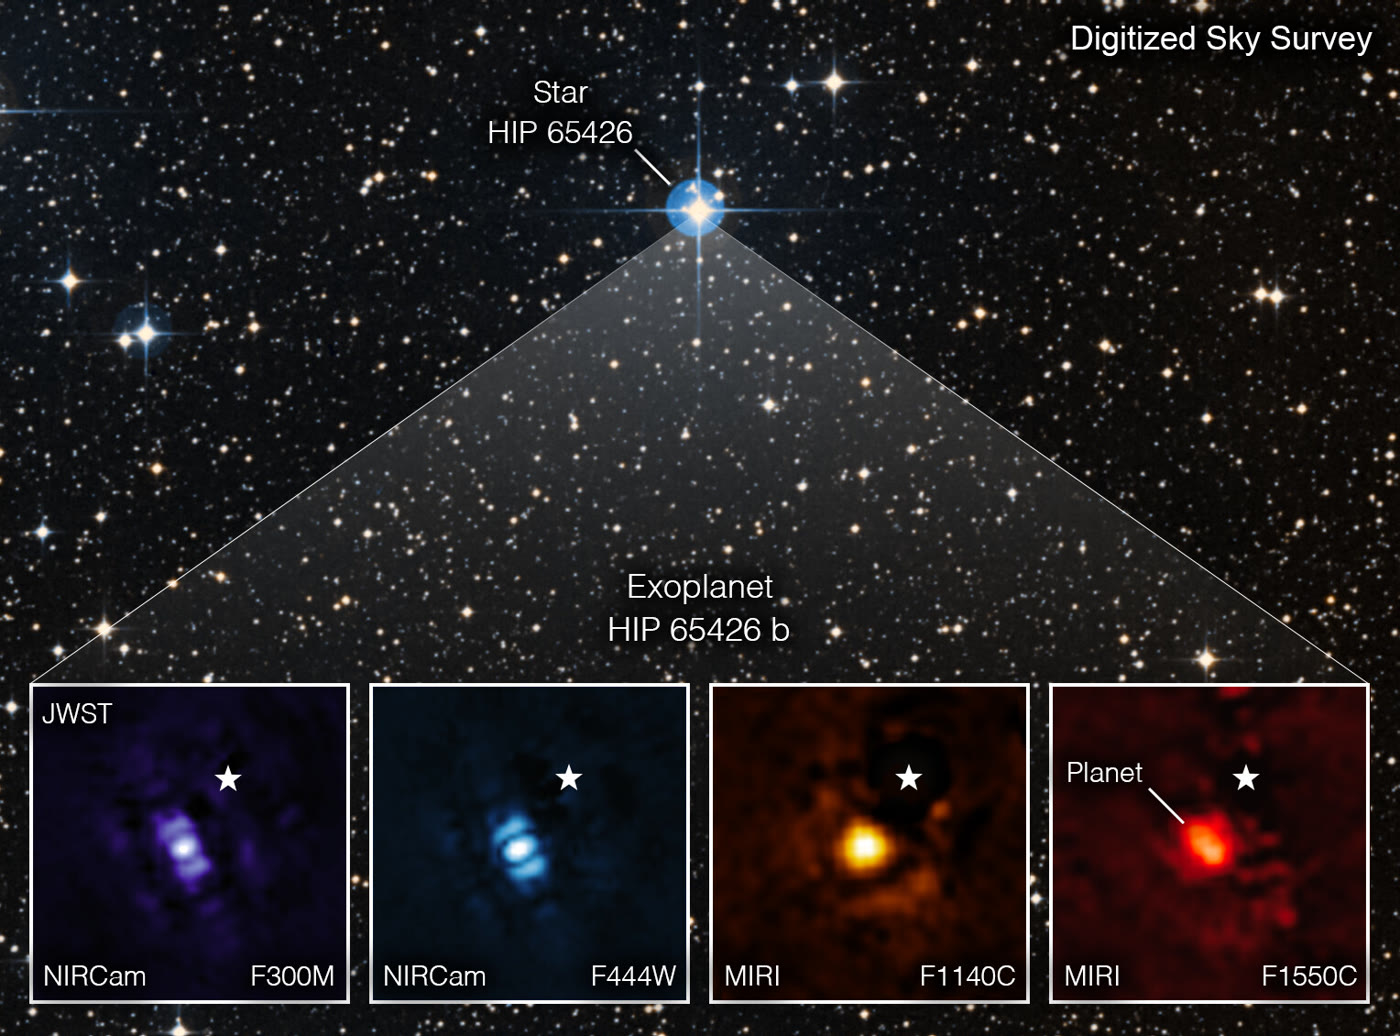
\includegraphics[width=0.86\linewidth]{images/book5/b3-hip65426b.jpg}
\par\smallskip{\small 詹姆斯·韦伯空间望远镜拍摄的首颗系外行星
HIP~65426~b，采用四个红外滤光片（下；上为
地面天空巡天中该恒星的视场）；恒星的光，
位于恒星符号所在位置处，已被
\omterm{def:b3:exoplanets:imaging}{日冕仪}挡住。该行星是一颗年轻的气态巨行星，
质量约为 6 至 8 个木星质量，年龄约 1500 万至 2000 万年，
与其恒星的距离约为地球与太阳距离的一百倍。图像：
NASA/ESA/CSA，A~Carter（UCSC），ERS~1386 团队，以及 A.~Pagan（STScI），
CC BY~4.0。}\label{fig:b3:exoplanets:hip65426}
\end{omfigure}
% ledger: photo:b3-hip65426b

第四种方法利用引力作透镜。当一颗恒星几乎恰好
经过另一颗更远的恒星前方时，其引力使背景恒星的光发生弯折，
并使其在数周内变亮；透镜星所带的行星
则会添加一个短暂的亮度脉冲。

\begin{definition}[引力微透镜；爱因斯坦半径]\label{def:b3:exoplanets:microlensing}
\emph{引力微透镜}\index{引力微透镜}是指
前景恒星（即透镜）靠近\omterm{def:b3:remote-sensing-gis:insar}{视线方向}经过时背景恒星暂时变亮的现象；
其所形成的像彼此靠得太近，无法分辨。
\emph{爱因斯坦半径}\index{爱因斯坦半径}是指
一个点透镜所能将光源弯成的环的角半径 $\theta_\mathrm E$，
其中透镜质量为 $M$、位于距离 $D_L$ 处，
将恰好位于其后方、距离为 $D_S$ 的光源弯成此环：
\[
\theta_\mathrm E = \sqrt{\frac{4GM}{c^2}\,\frac{D_S - D_L}{D_L D_S}} .
\]
\end{definition}

\begin{proposition}[点透镜放大率]\label{prop:b3:exoplanets:magnification}
与点透镜的角距离为 $u\,\theta_\mathrm E$ 的光源，
其亮度被放大的倍数为
\[
A(u) = \frac{u^2 + 2}{u\sqrt{u^2 + 4}} .
\]
\end{proposition}

\admitted

这两个结果都源于广义相对论中质量对光线的
弯折。对于质量为太阳质量一半、位于通往光源途中的透镜，
光源距离 \qty{8}{kpc}，$\theta_\mathrm E = \qty{0.71}{mas}$，爱因斯坦
环在透镜距离处的半径为 \qty{2.9}{au}。
当 $u = 1$ 时光源被增亮 1.34 倍，$u = 0.1$ 时增亮 10 倍。一颗
位于其恒星爱因斯坦环附近的行星会使
光变曲线产生一段短暂偏离。因此，微引力透镜可发现距其恒星几个天文单位的
冷行星，它们是\omterm{def:b3:exoplanets:transit}{凌星法}与\omterm{def:b3:exoplanets:rv}{视向速度法}所遗漏的，
但每次事件只发生一次，且不会重复出现。2003 年的一次事件
（次年发表）中，一段持续约 7 天的偏离
只能用质量为透镜质量 $\num{0.0039}$ 倍的伴天体来解释，
即一颗质量约为 1.5 个木星质量、距其恒星约
\qty{3}{au} 的行星。
% ledger: const:G, const:c, sun:mass, iau:parsec, const:au, bond04:ogle235

\begin{omfigure}
\centering
\begin{tikzpicture}[scale=0.95]
\fill (0,0) circle (0.06) node[below=2pt, font=\scriptsize] {光源};
\fill[omDef] (3.2,0) circle (0.09); \node[font=\scriptsize, omDef] at (3.2,-1.15) {透镜};
\draw[omDef] (3.2,0) ellipse (0.12 and 0.9);
\fill (6.4,0) circle (0.06) node[below=2pt, font=\scriptsize] {观测者};
\draw[thick, orange!80!black] (0,0) -- (3.2,0.9) -- (6.4,0);
\draw[thick, orange!80!black] (0,0) -- (3.2,-0.9) -- (6.4,0);
\draw[densely dashed, black!50] (6.4,0) -- (0,1.8) node[left, font=\scriptsize] {像};
\draw[densely dotted, black!50] (0,0) -- (6.4,0);
\draw[<->] (3.55,0) -- (3.55,0.9) node[midway, right, font=\scriptsize] {$R_\mathrm E$};
\draw[<->, black!60] (0,-1.5) -- (3.2,-1.5) node[midway, below, font=\scriptsize] {$D_S - D_L$};
\draw[<->, black!60] (3.2,-1.5) -- (6.4,-1.5) node[midway, below, font=\scriptsize] {$D_L$};
\end{tikzpicture}\hfill
\begin{tikzpicture}
\begin{axis}[width=0.48\linewidth, height=0.42\linewidth,
  xmin=-3, xmax=3, ymin=0.8, ymax=12, ymode=log,
  ytick={1,2,5,10}, yticklabels={1,2,5,10},
  xlabel={时间（$t_\mathrm E$）}, ylabel={放大率 $A$},
  tick label style={font=\scriptsize}, label style={font=\small},
  legend style={font=\scriptsize, at={(0.5,-0.30)}, anchor=north, legend columns=3, draw=none, cells={anchor=west}, /tikz/every even column/.append style={column sep=1em}}]
\addplot[thick, omDef] table[x=t_tE, y=A01] {figdata/out/bachelor-3-rv_transit-lens.dat};
\addlegendentry{$u_0 = 0.1$}
\addplot[thick, dashed, red!70!black] table[x=t_tE, y=A03] {figdata/out/bachelor-3-rv_transit-lens.dat};
\addlegendentry{$0.3$}
\addplot[thick, dotted, black] table[x=t_tE, y=A10] {figdata/out/bachelor-3-rv_transit-lens.dat};
\addlegendentry{$1$}
\end{axis}
\end{tikzpicture}
\par\smallskip{\small 左：引力透镜的几何示意，未按
比例绘制；来自光源的光线在约\omterm{def:b3:exoplanets:microlensing}{爱因斯坦半径}
$R_\mathrm E = \theta_\mathrm E D_L$ 处经过透镜，并到达观测者，观测者看到
光源被偏移后的像。右：点源经点透镜的放大率
随时间的变化，以透镜移动一个\omterm{def:b3:exoplanets:microlensing}{爱因斯坦半径}所用的时间
$t_\mathrm E$ 为单位，对应三种最小接近距离
$u_0$（以\omterm{def:b3:exoplanets:microlensing}{爱因斯坦半径}为单位）的情形。}\label{fig:b3:exoplanets:microlensing}
\end{omfigure}

各种方法各有其自身的偏差，已知行星的目录也
反映了这些偏差。\omterm{def:b3:exoplanets:rv}{视向速度法}偏向于探测距恒星较近的大质量行星；
\omterm{def:b3:exoplanets:transit}{凌星法}偏向于探测距恒星较近的大行星，并要求
轨道近乎处于\omterm{def:b3:remote-sensing-gis:insar}{视线方向}；微引力透镜法可发现几个天文单位远的行星；
\omterm{def:b3:exoplanets:imaging}{直接成像}法则发现位于数十乃至数百天文单位远处的年轻巨行星。
下图展示了这一结果：各种方法各占其自身的区域，
而太阳系行星大多落在它们之间的空位中。

\begin{dated}{2026}
2026 年 10 月 23 日，NASA Exoplanet Archive 收录了 6451 颗
已确认的行星。按发现方法统计：\omterm{def:b3:exoplanets:transit}{凌星法} 4785 颗，
\omterm{def:b3:exoplanets:rv}{视向速度法} 1204 颗，微引力透镜法 292 颗，\omterm{def:b3:exoplanets:imaging}{直接成像}法 98 颗，\omterm{def:b3:exoplanets:ttv}{凌星时间变化}
29 颗，其余由较罕见的方法发现，其中包括所有行星中最早发现的
几颗，于 1992 年围绕一颗脉冲星、借其脉冲的计时而发现。\omterm{def:b3:exoplanets:rv}{视向速度法}的
首次发现始于 1995 年，\omterm{def:b3:exoplanets:transit}{凌星法}始于 2002 年，
微引力透镜法和\omterm{def:b3:exoplanets:imaging}{直接成像}法始于 2004 年。
\end{dated}
% ledger: data:b5-pscomp

\begin{omfigure}
\centering
\begin{tikzpicture}
\begin{axis}[width=0.86\linewidth, height=0.56\linewidth,
  xmode=log, ymode=log, xmin=0.004, xmax=2000, ymin=0.02, ymax=1e5,
  legend image post style={scale=2.2},
  xlabel={半长轴（au）}, ylabel={质量或最小质量（$M_\oplus$）},
  tick label style={font=\scriptsize}, label style={font=\small},
  legend style={font=\scriptsize, at={(0.5,-0.20)}, anchor=north, legend columns=4, draw=none, cells={anchor=west}, /tikz/every even column/.append style={column sep=1em}}]
\addplot[only marks, mark=*, mark size=0.6pt, omDef, opacity=0.6] table[x=a_au, y=mass] {figdata/out/bachelor-3-exoplanet_archive-ma-tr.dat};
\addlegendentry{凌星法}
\addplot[only marks, mark=*, mark size=0.6pt, red!70!black, opacity=0.6] table[x=a_au, y=mass] {figdata/out/bachelor-3-exoplanet_archive-ma-rv.dat};
\addlegendentry{视向速度法}
\addplot[only marks, mark=triangle*, mark size=1.2pt, green!45!black] table[x=a_au, y=mass] {figdata/out/bachelor-3-exoplanet_archive-ma-ml.dat};
\addlegendentry{微引力透镜法}
\addplot[only marks, mark=diamond*, mark size=1.5pt, orange!85!black] table[x=a_au, y=mass] {figdata/out/bachelor-3-exoplanet_archive-ma-im.dat};
\addlegendentry{直接成像法}
\addplot[only marks, mark=square*, mark size=1.6pt, black, forget plot] table[x=a_au, y=mass] {figdata/out/bachelor-3-exoplanet_archive-solar.dat};
\node[font=\scriptsize, anchor=west, fill=white, inner sep=1pt] at (axis cs:1.15,1.0) {地球};
\node[font=\scriptsize, anchor=east, fill=white, inner sep=1pt] at (axis cs:0.63,0.82) {金星};
\node[font=\scriptsize, anchor=east, fill=white, inner sep=1pt] at (axis cs:0.34,0.055) {水星};
\node[font=\scriptsize, anchor=west, fill=white, inner sep=1pt] at (axis cs:1.75,0.107) {火星};
\node[font=\scriptsize, anchor=west, fill=white, inner sep=1pt] at (axis cs:6.0,318) {木星};
\node[font=\scriptsize, anchor=west, fill=white, inner sep=1pt] at (axis cs:11,95) {土星};
\node[font=\scriptsize, anchor=north, fill=white, inner sep=1pt] at (axis cs:25,11) {天王星、海王星};
\end{axis}
\end{tikzpicture}
\par\smallskip{\small 已确认的行星，其质量（或\omterm{def:b3:exoplanets:rv}{最小质量}）
与半长轴均已测得，按发现方法统计（NASA Exoplanet
Archive，2026 年 10 月 23 日：\omterm{def:b3:exoplanets:transit}{凌星法} 1691 颗，\omterm{def:b3:exoplanets:rv}{视向速度法} 1151 颗，微引力透镜法 286
颗，\omterm{def:b3:exoplanets:imaging}{直接成像}法 94 颗），并标出太阳系行星（黑色
方块）。由\omterm{def:b3:exoplanets:mass-radius}{质量–半径关系}推算的质量未予列入。本研究
使用了 NASA Exoplanet Archive，该档案由
加州理工学院运营，依据与美国国家航空航天局
签订的合同，依托 Exoplanet Exploration
Program 计划进行。}\label{fig:b3:exoplanets:methods}
\end{omfigure}
% ledger: data:b5-pscomp, planet:Mercury.mass, planet:Venus.mass, planet:Earth.mass, planet:Mars.mass, planet:Jupiter.mass, planet:Saturn.mass, planet:Uranus.mass, planet:Neptune.mass, planet:Mercury.dist, planet:Venus.dist, planet:Earth.dist, planet:Mars.dist, planet:Jupiter.dist, planet:Saturn.dist, planet:Uranus.dist, planet:Neptune.dist

\section{已有发现}\label{sec:b3:exoplanets:found}

最令人意外的首个发现是\omterm{def:b3:exoplanets:classes}{热木星}，
即轨道仅为几天的巨行星。51~Pegasi~b 不可能在离恒星如此近的地方形成；
它应当形成于更远处，或许在几个天文单位处，
位于原行星盘的雪线之外，随后通过与盘的相互作用向内迁移，
正如理论所预言的那样。
% ledger: nobel19:migration

\begin{definition}[热木星；超级地球；亚海王星]\label{def:b3:exoplanets:classes}
称\emph{热木星}\index{热木星}为轨道较近的巨行星，
通常取其\omterm{def:b3:exoplanets:rv}{最小质量}大于 0.1 个木星质量，且周期
短于 10 天。称\emph{超级地球}\index{超级地球}为
比地球大但小于\omterm{def:b3:exoplanets:radius-valley}{半径谷}的行星，即半径至多
约 1.5 至 2 个地球半径，因而很可能是岩质的。称\emph{亚海王星}\index{亚海王星}为
位于\omterm{def:b3:exoplanets:radius-valley}{半径谷}之上、小于海王星的行星，半径约为 2 至
4 个地球半径，其半径要求存在由轻质气体
或挥发物构成的包层。
\end{definition}
% ledger: wright12:hj, fulton17:gap, planet:Neptune.diameter, planet:Earth.diameter

\begin{definition}[出现率]\label{def:b3:exoplanets:occurrence}
某一类行星的\emph{出现率}\index{出现率}是指
平均每颗恒星所拥有的此类行星数，或拥有此类行星的恒星所占比例，
拥有此类行星者，在给定尺寸（或质量）与周期范围内，经
对巡天计数进行修正，扣除其无法探测的行星：
即轨道取向不利于凌星的行星，以及过小
或过远而无法被观测到的行星。
\end{definition}

\omterm{def:b3:exoplanets:classes}{热木星}在星表中十分醒目，因其最易被找到，
但它们实际很罕见：一项针对附近类太阳恒星的视向速度巡天发现，
此类行星存在于 \qty[separate-uncertainty=true]{1.2 \pm 0.38}{\percent} 的恒星周围。小型行星很常见。
对开普勒空间望远镜所观测的 \num{42000} 颗恒星的光变曲线进行搜索，
一项研究发现 603 颗行星，其中 10 颗与地球大小相近（半径为 1 至 2
个地球半径），接收的太阳光为地球的 1 至 4 倍；
经凌星概率及搜索遗漏行星的修正，
约 \qty[separate-uncertainty=true]{11 \pm 4}{\percent} 的类太阳恒星拥有这样的
行星。
% ledger: wright12:hj, petigura13:eta

小型行星的尺寸分布并不均匀。在经过精确测量的近轨道行星中，
半径为 1.5 至 2.0 个地球半径者，
其数量至少只有刚好略小或略大者的一半。

\begin{definition}[半径谷]\label{def:b3:exoplanets:radius-valley}
\emph{半径谷}\index{半径谷}是指在
周期短于约 100 天的行星中，半径约介于
1.5 至 2.0 个地球半径之间的行星数量的亏缺；它将\omterm{def:b3:exoplanets:classes}{超级地球}
与\omterm{def:b3:exoplanets:classes}{亚海王星}分隔开来。
\end{definition}
% ledger: fulton17:gap

这一亏缺被解释为逃逸的痕迹。岩质内核形成时带有
仅占其质量几个百分点的氢氦包层，其半径为
裸露内核的两倍。在年轻而活跃的恒星附近，这样的
包层会因\omterm{def:b3:planetary-atmospheres:hydrodynamic}{流体动力学逃逸}而被加热并损失：一是恒星的
高能辐射（在最初 1 亿年内）
（光致蒸发），二是冷却内核自身释放的热量（核心驱动
质量损失）。模型将行星聚集为半径约 1.3 个地球半径的
裸露内核，以及两倍于此尺寸的行星；两者之间的行星很少。这两种
机制对恒星的依赖方式不同，因而围绕不同类型恒星的行星
或可将二者区分开来。
% ledger: owen17:valley, ginzburg18:core-powered

\begin{omfigure}
\centering
\begin{tikzpicture}
\begin{axis}[name=pr, width=0.50\linewidth, height=0.50\linewidth,
  xmode=log, ymode=log, xmin=1, xmax=100, ymin=0.8, ymax=4,
  ytick={1,1.5,2,3,4}, yticklabels={1,1.5,2,3,4},
  xlabel={周期（天）}, ylabel={半径（$R_\oplus$）},
  tick label style={font=\scriptsize}, label style={font=\small},
  title={(a)}, title style={font=\small}]
\fill[black!10] (axis cs:1,1.5) rectangle (axis cs:100,2.0);
\addplot[only marks, mark=*, mark size=0.5pt, omDef, opacity=0.7] table[x=period, y=radius] {figdata/out/bachelor-3-exoplanet_archive-pr.dat};
\end{axis}
\begin{axis}[at={(pr.east)}, anchor=west, xshift=0.09\linewidth,
  width=0.42\linewidth, height=0.50\linewidth,
  xmode=log, xmin=0.8, xmax=4, ymin=0, ymax=185,
  xtick={1,1.5,2,3,4}, xticklabels={1,1.5,2,3,4},
  xlabel={半径（$R_\oplus$）}, ylabel={行星数},
  tick label style={font=\scriptsize}, label style={font=\small},
  title={(b)}, title style={font=\small}]
\fill[black!10] (axis cs:1.5,0) rectangle (axis cs:2.0,185);
\addplot[const plot mark left, thick, omDef, fill=omDef!25] table[x=r, y=n] {figdata/out/bachelor-3-exoplanet_archive-histstep.dat} \closedcycle;
\end{axis}
\end{tikzpicture}
\par\smallskip{\small (a)~半径已知精度优于
\qty{10}{\percent}的凌星行星，围绕小于两个太阳半径的恒星，周期为
1 至 100 天（共 2370 颗行星，NASA Exoplanet Archive，
2026 年 10 月 23 日）；阴影为 1.5 至 2.0 个地球半径的\omterm{def:b3:exoplanets:radius-valley}{半径谷}。
(b)~对同样的行星，在 $\log R$ 上等宽划分为 20 个区间进行计数。
计数未对巡天遗漏的行星作修正，这些被遗漏者
在小型行星中更为众多；但谷形依然清晰可见。}\label{fig:b3:exoplanets:valley}
\end{omfigure}
% ledger: data:b5-pscomp, fulton17:gap

\begin{definition}[质量–半径关系]\label{def:b3:exoplanets:mass-radius}
某一成分的\emph{质量–半径关系}\index{质量–半径关系}是指
该成分行星的半径作为其质量的函数，
由其材料在静力平衡下的状态方程算得；
将实测行星与候选成分的
关系进行比较。
\end{definition}

岩质行星受自身重力压缩，其半径增长
慢于 $M^{1/3}$。以地球地震模型为基础构建的双层行星模型，
经拟合得 $R/R_\oplus = (1.07 - 0.21\,C)
(M/M_\oplus)^{1/3.7}$，适用于 1 至 8 个地球质量，核质量分数
$C$ 的范围为 0 至 0.4；以地球、金星及少数小型
系外行星为拟合对象，得 $C = 0.26 \pm 0.07$。
同质量下铁质行星更小；一半为水的行星则更大；
仅占其质量 \qty{2}{\percent} 的氢包层，使一颗
质量为 5 个地球质量、直径为 \num{2.6} 个地球半径的行星，
其大小与\omterm{def:b3:exoplanets:classes}{亚海王星}相当。简并度是真实存在的：半径与质量只给出一个密度，
而若干种铁、岩石、水和气体的混合物可以共享这一密度。
岩质行星开普勒-10~b 质量为 3.24 个地球质量、半径为 1.47 个地球半径，
平均密度为 \qty{5.6}{g.cm^{-3}}；气态巨行星 WASP-39~b，
质量为 89 个地球质量、半径为 14.3 个地球半径，密度为 \qty{0.17}{g.cm^{-3}}。
% ledger: zeng16:rocky, data:b5-zeng, data:b5-pscomp

\begin{omfigure}
\centering
\begin{tikzpicture}
\begin{axis}[width=0.86\linewidth, height=0.58\linewidth,
  xmode=log, ymode=log, xmin=0.3, xmax=5000, ymin=0.5, ymax=25,
  ytick={0.5,1,2,4,10,20}, yticklabels={0.5,1,2,4,10,20},
  xlabel={质量 ($M_\oplus$)}, ylabel={半径 ($R_\oplus$)},
  tick label style={font=\scriptsize}, label style={font=\small},
  legend style={font=\scriptsize, at={(0.5,-0.20)}, anchor=north, legend columns=3, draw=none, cells={anchor=west}, /tikz/every even column/.append style={column sep=1em}}]
\addplot[only marks, mark=*, mark size=0.6pt, black!35, forget plot] table[x=mass, y=radius] {figdata/out/bachelor-3-exoplanet_archive-mr.dat};
\addplot[thick, black] table[x=mass, y=radius] {figdata/out/bachelor-3-exoplanet_archive-zeng-iron.dat};
\addlegendentry{纯铁}
\addplot[thick, brown!70!black] table[x=mass, y=radius] {figdata/out/bachelor-3-exoplanet_archive-zeng-earthlike.dat};
\addlegendentry{类地岩石}
\addplot[thick, omDef] table[x=mass, y=radius] {figdata/out/bachelor-3-exoplanet_archive-zeng-water50.dat};
\addlegendentry{50\,\% 水}
\addplot[thick, dashed, orange!85!black] table[x=mass, y=radius] {figdata/out/bachelor-3-exoplanet_archive-zeng-h2-2pc.dat};
\addlegendentry{岩石 + 2\,\% 氢}
\addplot[only marks, mark=square*, mark size=1.8pt, red!70!black] table[x=mass, y=radius] {figdata/out/bachelor-3-exoplanet_archive-solar.dat};
\addlegendentry{太阳系}
\node[font=\scriptsize, anchor=north west] at (axis cs:1.05,0.97) {地球};
\node[font=\scriptsize, anchor=south east] at (axis cs:0.80,0.97) {金星};
\node[font=\scriptsize, anchor=south east, fill=white, inner sep=1pt] at (axis cs:13.5,4.3) {天王星、海王星};
\node[font=\scriptsize, anchor=east, fill=white, inner sep=1pt] at (axis cs:80,9.45) {土星};
\node[font=\scriptsize, anchor=north, fill=white, inner sep=1pt] at (axis cs:318,10.3) {木星};
\end{axis}
\end{tikzpicture}
\par\smallskip{\small 1078 颗凌日行星的质量与半径，
其质量测定精度优于 \qty{25}{\percent}，半径测定精度优于 \qty{10}{\percent}
（灰色点；NASA 系外行星档案，2026 年 10 月 23 日），
并附 L.~Zeng 等人（2016，2019）的模型曲线：纯铁；
类地岩石，三分之一为铁、三分之二为硅酸盐；此类地核之上覆以一半为水，
温度 \qty{500}{K}；类地地核外包氢包层，其质量
占其质量的 \qty{2}{\percent}，温度 \qty{500}{K}。红色方块：太阳系行星
（水星与火星位于图的左侧，超出范围
）。}\label{fig:b3:exoplanets:mass-radius}
\end{omfigure}
% ledger: data:b5-pscomp, data:b5-zeng, planet:Earth.mass, planet:Earth.diameter, planet:Venus.mass, planet:Venus.diameter, planet:Jupiter.mass, planet:Jupiter.diameter, planet:Saturn.mass, planet:Saturn.diameter, planet:Uranus.mass, planet:Uranus.diameter, planet:Neptune.mass, planet:Neptune.diameter

\section{大气}\label{sec:b3:exoplanets:atmospheres}

凌日行星既可以称重和测量，也可以“嗅”其成分。
凌日期间，行星大气的一圈薄环位于恒星前方，
星光穿过该环而被滤去。在大气中某种气体吸收的波长上，
较高处的薄环不透明，
行星看起来更大。

\begin{definition}[透射光谱法；次食]\label{def:b3:exoplanets:transmission}
\emph{透射光谱法}\index{透射光谱法}测量
凌日深度随波长的变化，以探测恒星光穿过行星边缘的大气所含气体。
\emph{次食}\index{次食}是
行星运行到恒星背后的过程，
在圆轨道上发生于凌日后半个轨道周期；
此时系统通量的下降可测得
行星白昼一面的光。
\end{definition}

\begin{proposition}[透射信号]\label{prop:b3:exoplanets:transmission}
标高为 $H \ll R_p$ 的大气，在吸收带的波长处，其不透明层
比邻近波长多出 $n$ 个标高的厚度，
则该处凌日深度增加
\[
\Delta\delta \approx n\,\frac{2HR_p}{R_\star^2} .
\]
\end{proposition}

\begin{proof}
行星的视半径由 $R_p$ 增至 $R_p + nH$，
故深度 $(R_p + nH)^2/R_\star^2$ 增加 $(2nHR_p + n^2H^2)/R_\star^2$，
其值为 $2nHR_p/R_\star^2$，当 $nH \ll R_p$ 时成立。
\end{proof}

标高 $H = kT/\bar m g$ 对于低重力、轻氢大气的炽热行星很大，
对于大气厚重的低温致密行星则很小。
以地球对着太阳观测为例，取 $H = \qty{8}{km}$，
每个标高使深度增加百万分之 0.2；对于炽热、膨胀的气态巨行星，
则可达百万分之数百。
% ledger: planet:Earth.diameter, sun:R

\begin{proposition}[次食深度]\label{prop:b3:exoplanets:eclipse}
若行星的白昼一面按温度 $T_d$ 的黑体辐射，
恒星按温度 $T_\star$ 的黑体辐射，
则波长 $\lambda$ 处的\omterm{def:b3:exoplanets:transmission}{次食}深度为
\[
\delta_\mathrm{ecl} \approx \left(\frac{R_p}{R_\star}\right)^2
  \frac{B_\lambda(T_d)}{B_\lambda(T_\star)},
\]
其中 $B_\lambda$ 为普朗克定律，略去行星的反射光。
\end{proposition}

\begin{proof}
食前，观测者接收到的恒星光与
$\pi R_\star^2 B_\lambda(T_\star)$ 成正比，
另加白昼一面的光，与 $\pi R_p^2 B_\lambda(T_d)$ 成正比；
食时则只有恒星的光。相对下降量为行星项与恒星项之比，
因行星很小。
\end{proof}

\omterm{def:b3:exoplanets:transmission}{次食}在红外波段最深，此时低温行星相对其恒星最亮：
它给出白昼一面的温度，
若白昼一面炽热而夜间一面低温，说明大气稀薄或不存在，
无法将热量输送开来。

\begin{dated}{2023}
2022 年，气态巨行星 WASP-39~b 的透射光谱，
由詹姆斯·韦伯太空望远镜在 3.0 至 \qty{5.5}{\micro m} 之间测得，
显示出显著的二氧化碳吸收带，位于 \qty{4.3}{\micro m} 处，
达 26 个标准差；此前的测光仅隐约提示过该气体，
这是该气体首次在系外行星大气中被明确证认。
2023 年，对地球大小的 TRAPPIST-1~b 测得五次\omterm{def:b3:exoplanets:transmission}{次食}，
该行星从一颗低温小恒星接收到的日光为地球的四倍，
测得波长为 \qty{15}{\micro m}。这些数据
仅能由白昼一面再辐射的热量解释，
未探测到二氧化碳：该行星几乎没有大气，
无法将热量输送到夜间一面。
\end{dated}
% ledger: jwst23:wasp39-co2, greene23:trappist1b

小恒星宜居带内的岩质行星，
在这一极限上已处于这些方法的探测范围之内。它们在前一章所述的
逃逸过程中是否保住了大气，
如今已成为一个观测问题。

\section{练习}

\begin{exercise}[$\star$]\label{exo:b3:exoplanets:1}
(a)~计算木星与地球各自引起的太阳视向速度半振幅。
木星（质量 \qty{1898e24}{kg}，周期 \num{4331}~天，偏心率 0.049）
和地球（质量 \qty{5.97e24}{kg}，周期 \num{365.2}~天，
偏心率 0.017）。太阳质量为 \qty{1.9884e30}{kg}。
(b)~将精度 \qty{3.5}{km/h} 和 \qty{0.35}{km/h} 换算为米每秒，
并加以比较。
\end{exercise}

\begin{exercise}[$\star$]\label{exo:b3:exoplanets:2}
(a)~计算木星（半径 \qty{71492}{km}）和地球（半径 \qty{6378}{km}）
相对太阳（半径 \qty{695700}{km}）的\omterm{def:b3:exoplanets:transit}{凌星深度}。
(b)~对轨道半径分别为 \num{778.5} 和 \qty{149.6}{\mega km} 的
两颗行星，计算随机放置的观测者
看到其各自凌日的概率。
\end{exercise}

\begin{exercise}[$\star$]\label{exo:b3:exoplanets:3}
51~Pegasi~b 使其恒星产生的视向速度半振幅为
\qty{59}{m.s^{-1}}，周期为 \qty{4.23}{d}。取恒星质量等于太阳质量，
求该行星的\omterm{def:b3:exoplanets:rv}{最小质量}（分别以木星质量和地球质量表示）
以及其轨道半径。
\end{exercise}

\begin{exercise}[$\star$]\label{exo:b3:exoplanets:4}
一颗质量为半个太阳质量的恒星位于 \qty{4}{kpc} 处，
透镜化了位于 \qty{8}{kpc} 处的一颗恒星（$\qty{1}{pc} = \qty{3.0857e16}{m}$）。
(a)~以毫角秒为单位计算其\omterm{def:b3:exoplanets:microlensing}{爱因斯坦半径}，并以天文单位计算
透镜距离处的爱因斯坦环半径。(b)~计算
$u = 1$、$0.5$ 和 $0.1$ 时的放大率。(c)~若透镜以
\qty{200}{km.s^{-1}} 的速度沿\omterm{def:b3:remote-sensing-gis:insar}{视线方向}运动，
它穿过一个\omterm{def:b3:exoplanets:microlensing}{爱因斯坦半径}需要多长时间？
\end{exercise}

\begin{exercise}[$\star\star$]\label{exo:b3:exoplanets:5}
一颗行星的半径比为 $p = 0.12$，
绕一颗质量为一个太阳质量、半径为一个太阳半径的恒星运行，周期为 \qty{3.0}{d}。(a)~计算 $a/R_\star$。(b)~计算
$T_{14}$ 和 $T_{23}$，分别对应 $b = 0$ 与 $b = 0.7$ 的情形，
并求第二种情形下的倾角。(c)~光变曲线的形状如何区分
中心凌日与掠过凌日？
\end{exercise}

\begin{exercise}[$\star\star$]\label{exo:b3:exoplanets:6}
利用系外行星档案中的质量和半径，计算
TRAPPIST-1~b（1.374 个地球质量，1.116 个地球半径）、
开普勒-10~b（3.24，1.47）、WASP-39~b（89.31，14.34）和
HD~209458~b（232.0，15.58），取 $M_\oplus = \qty{5.97e24}{kg}$，$R_\oplus =
\qty{6378}{km}$。哪些是岩质行星，哪些是气态行星？
\end{exercise}

\begin{exercise}[$\star\star$]\label{exo:b3:exoplanets:7}
一颗恒星有一颗轨道偏心的行星，其视向速度
从 $+\qty{50.4}{m.s^{-1}}$ 变化到 $-\qty{9.6}{m.s^{-1}}$，系统质心的速度为
\qty{12.4}{m.s^{-1}}。利用该定理的偏心形式，
计算 $K$ 和 $e\cos\omega$。
为什么两个极值的平均值可能不等于 $\gamma$？
\end{exercise}

\begin{exercise}[$\star\star$]\label{exo:b3:exoplanets:8}
WASP-39~b 的质量为 89.31 个地球质量，半径为 14.34 个地球半径；
其恒星的半径为 0.939 个太阳半径。取其大气温度为 \qty{1100}{K}，
平均分子质量为 \qty{2.3}{u}。(a)~计算其表面重力、标高和\omterm{def:b3:exoplanets:transit}{凌星深度}。
(b)~计算一个标高的透射信号，
以及高度为两个标高的吸收带的透射信号，
并以百万分之一计。
\end{exercise}

\begin{exercise}[$\star\star$]\label{exo:b3:exoplanets:9}
TRAPPIST-1~b 的半径为 1.116 个地球半径；其恒星的半径为 0.1192 个太阳半径，
温度为 \qty{2566}{K}。计算该行星在 \qty{15}{\micro m} 处的\omterm{def:b3:exoplanets:transmission}{次食}深度，
对白昼一面温度为 \qty{400}{K} 和 \qty{500}{K} 的情形分别计算，
（$hc/k = \qty{0.014388}{m.K}$）。
为什么对\omterm{def:b3:exoplanets:transmission}{次食}深度的测量可以作为一支温度计？
\end{exercise}

\begin{exercise}[$\star\star\star$]\label{exo:b3:exoplanets:10}
一颗虚构的红矮星质量为 0.2 个太阳质量，半径为 0.2 个太阳半径，
光度为 \num{0.005} 个太阳光度。(a)~行星在何距离处接收到与地球
相同的恒星通量？其周期是多少？(b)~若该处有一颗质量为一个地球质量的行星，
计算其引起的半振幅，并与地球对太阳的效应相比较。(c)~
计算一颗地球大小行星的\omterm{def:b3:exoplanets:transit}{凌星深度}。
为什么这类恒星在寻找宜居带岩质行星时
是优先的目标？
\end{exercise}

\begin{exercise}[$\star\star\star$]\label{exo:b3:exoplanets:11}
对于二次型\omterm{def:b3:exoplanets:limb}{临边昏暗}定律，证明圆面的平均强度为
$I(1)(1 - u_1/3 - u_2/6)$。由此推导，
以 $p^2$ 为单位，求小型行星位于 $r = 0$、$0.5$ 和 $0.9$ 处时的\omterm{def:b3:exoplanets:transit}{凌星深度}，取 $u_1 = 0.40$，
$u_2 = 0.25$。若采用均匀圆面模型，对于在凌日中点观测到的 $b = 0$ 的行星，
其半径会产生多大的误差？
\end{exercise}

\begin{exercise}[$\star\star\star$]\label{exo:b3:exoplanets:12}
一项巡天观测了 \num{42000} 颗类太阳恒星，搜寻接收到地球日光的
一至四倍（即轨道位于 0.5 至 \qty{1}{au} 之间）的地球大小行星。
(a)~计算在 0.5、0.7 和 \qty{1}{au} 处的凌日概率。
(b)~若 \qty{11}{\percent} 的恒星在约 \qty{0.7}{au} 处拥有一颗这样的行星，
则其中有多少颗会凌日？
(c)~该巡天共发现十颗。这一差异度量了什么？
为何\omterm{def:b3:exoplanets:occurrence}{出现率}必须针对它加以修正？
\end{exercise}

\section{问题：塞勒涅之灯周围的行星}

\begin{problem}[{周末问题——称重、测径与嗅探一颗
虚构行星}]
\label{pb:b3:exoplanets:1}
塞勒涅之灯是一颗虚构的 K~矮星，质量为 0.80 个太阳质量，半径
为 0.76 个太阳半径，有效温度为 \qty{5000}{K}。一项
径向速度巡天发现其速度随时间呈正弦变化，
周期为 \qty{12.0}{d}，半振幅为 \qty{2.59}{m.s^{-1}}。一台
太空望远镜随后观测到相同周期的凌日，凌日深度为
百万分之 \num{838}，总时长 $T_{14} = \qty{3.23}{h}$。
取 $M_\odot = \qty{1.9884e30}{kg}$，$R_\odot = \qty{695700}{km}$，
$L_\odot = \qty{3.828e26}{W}$, $M_\oplus = \qty{5.97e24}{kg}$,
$R_\oplus = \qty{6378}{km}$.

\medskip\noindent\textbf{第一部分——径向速度。}
\begin{enumerate}
\item 求轨道半径，分别以米和天文单位表示，
  忽略行星质量相对于恒星质量的贡献。
\item 求行星的轨道速度。
\item 求行星的\omterm{def:b3:exoplanets:rv}{最小质量}，以地球质量为单位。
\item 求恒星绕质心运动的轨道半径，
  并检验其是否与观测到的半振幅相符。
\item 信号幅度超过精度
  \qty{1}{m.s^{-1}} 与 \qty{0.1}{m.s^{-1}} 的多少倍？
\item 若轨道偏心率为 $e = 0.2$ 而 $K$ 不变，
  则\omterm{def:b3:exoplanets:rv}{最小质量}将改变多少？
\end{enumerate}

\medskip\noindent\textbf{第二部分——凌日。}
\begin{enumerate}[resume]
\item 求半径比 $p = R_p/R_\star$。
\item 求行星半径，分别以千米和地球半径为单位。
\item 求 $a/R_\star$。
\item 求正中心凌日（$b = 0$）的时长。
\item 由观测所得的 $T_{14}$，求\omterm{def:b3:exoplanets:transit}{碰撞参数}。
\item 求轨道倾角。
\item 若从随机方向观测，该行星凌日的
  概率为多少？
\end{enumerate}

\medskip\noindent\textbf{第三部分——它由什么构成？}
\begin{enumerate}[resume]
\item 求行星的真实质量。
\item 求其平均密度。
\item 在类地岩质模型曲线上，质量与之相同的行星
  半径应为 1.74 个地球半径。将二者加以比较，并说明
  该行星除岩石外还必须含有什么。
\item 该行星相对于\omterm{def:b3:exoplanets:radius-valley}{半径谷}位于何处？它是
  \omterm{def:b3:exoplanets:classes}{超级地球}还是\omterm{def:b3:exoplanets:classes}{亚海王星}？
\item 求其表面重力加速度。
\end{enumerate}

\medskip\noindent\textbf{第四部分——它的大气。}
\begin{enumerate}[resume]
\item 求恒星的光度，分别以瓦特和太阳
  光度表示。
\item 求行星所接收的恒星通量相对于地球的
  比值。该行星是否位于宜居带？
\item 取邦德反照率为 0.3，求其平衡温度。
\item 求由氢和氦组成的大气在该温度下的标高
  （平均分子质量为 \qty{2.3}{u}）。
\item 求高为一个标高时的透射信号，以及
  高为两个标高的水吸收带的透射信号，以百万分率计。
\item 对水蒸气大气（平均分子质量 \qty{18}{u}）求同样的量，
  两者中哪一种能被精度约为百万分之十的太空望远镜
  与平坦光谱区分开来？
\item 以克每立方厘米为单位，给出行星的平均密度，
  保留两位有效数字。
\end{enumerate}
\end{problem}
% ledger: sun:mass, sun:R, sun:L, planet:Earth.mass, planet:Earth.diameter, const:G, const:kB, const:sigma, nist:u, data:b5-zeng, fulton17:gap, eso:espresso
